\subsection{Background Subtraction}
\label{subsection:training}
Background subtraction is the first step is determining which pixels of an image belong to a vehicle and divides all pixels in an image into two groups, foreground and background. This background subtraction implementation uses a clustering method known as a Mixture of Gaussian or Gaussian Mixture Model (\ref{subsection:mog}). 

Background subtraction is the most complex and thus the most computationally expensive part of the detection process. It is imperative, however, that the algorithm be fast enough to process images in real-time, such that traffic data is reflect live conditions. Fortunately the OpenCV's BackgroundSubtractorMOG2 function \cite{opencv_mog2} is both fast and effective making it a suitable choice for a low power microcontroller. OpenCV's implementation is based on the the research by Zoran Zivkovic and Ferdinand van der Heijden \cite{zivkovic_pattern_recognition} \cite{zivkovic_heijden_pattern_recognition_letters} which takes only pixel colours as input.

Figure \ref{fig:example_subtraction} shows the application of the background subtractor on an arbitrary traffic image highlighting its ability to isolate, in particular, moving objects. Movement changes the value of pixels over a short time scale making it easy for the model to detect them as foreground objects. Shadows also register as a foreground objects but fortunately OpenCV's implementation is able to explicitly detect shadows and present them as gray pixels in the resulting foreground mask. In Figure \ref{fig:foreground_mask_filtered} the gray pixels in and around the white foreground objects are shadows which are removed via thresholding (equation \ref{eq:threshold}). 

\subsubsection{Calibration}

OpenCV's Gaussian Mixture Model (GMM) implementation has two important parameters to consider, \emph{history} and \emph{shadows}, where history is an integer and shadows is a Boolean. 

The history parameter determines how many formerly processed images affect the Gaussian Mixture Model, for example, if the subtractor's history is 500 and it processes 501 images then the 1st image no longer has influence on the subtractor's models but the 501st does. For a 30fps video 500 images is only about 16 seconds, therefore if a vehicle stops for that long its presence will be completely reflected in the cluster models. In Figure \ref{fig:cluster_adaptation} the vehicles in the third lane are stationary for sufficiently long to be absorbed into the background by the GMM, this is not an issue as when they move again they are recognized once more. Thus, the history length should be long enough to absorb small but consistent changes in pixel values, like swaying tree branches, into the background but short enough that a slowly moving vehicle registers as a foreground object. In short the longer the history the more insensitive the background model becomes to change.

The shadows parameter tells the model if a cluster for shadows should be specified, if they are they appear as gray, not white, in the foreground mask. In this system's implementation they are set to true as it allows them to be removed from the foreground mask, Figures \ref{fig:foreground_mask_unfiltered} and \ref{fig:thresh_shadow} show their presence and consequent removal via thresholding. 

Finally, the subtractor when initialized hasn't had a chance to develop cluster models for the given traffic scene resulting foreground mask with a lot of anomalies. By 'training' the model on a few seconds of video before using it to collect traffic data any initial erroneous readings are avoided. This simply involves feeding the algorithm a few hundred images before using it to collect data.

\begin{figure}[H]
	\centering
	\begin{subfigure}[b]{0.4\linewidth}
        \centering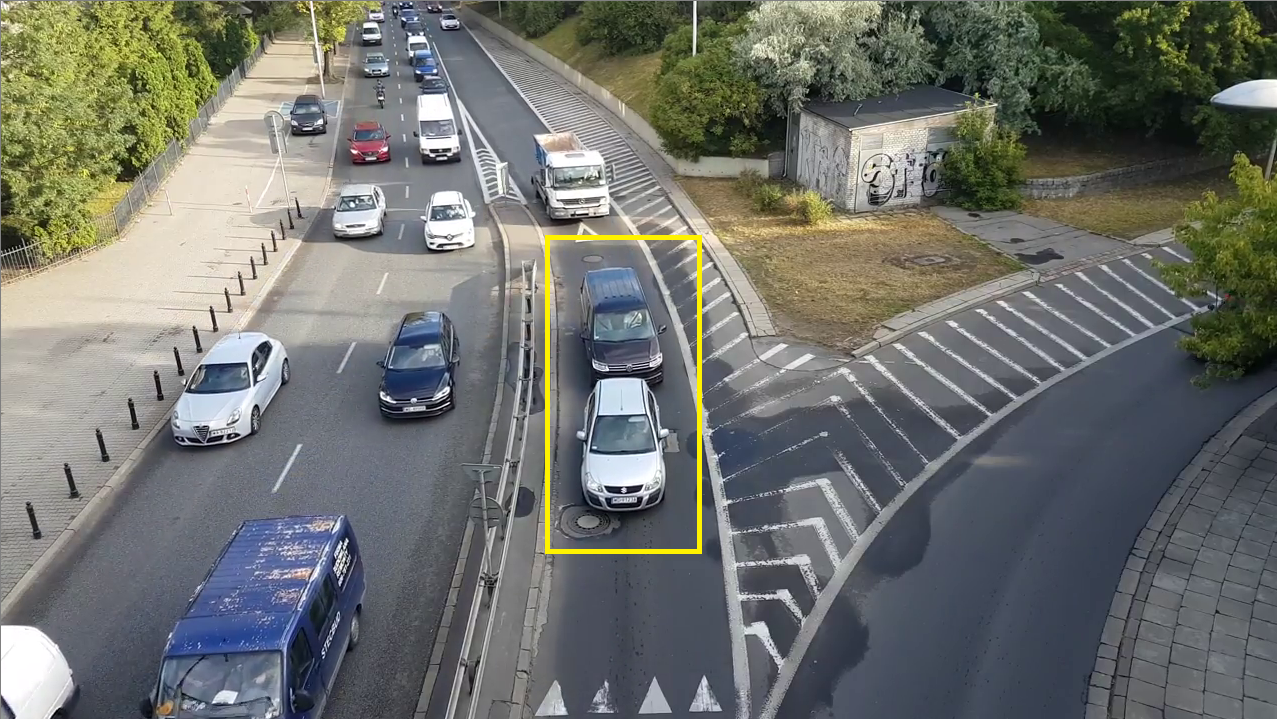
\includegraphics[width = \textwidth]{design/detection/calibration/original}
        \caption{Original Frame - vehicles moving.}
    \end{subfigure}%
    \begin{subfigure}[b]{0.4\linewidth}
        \centering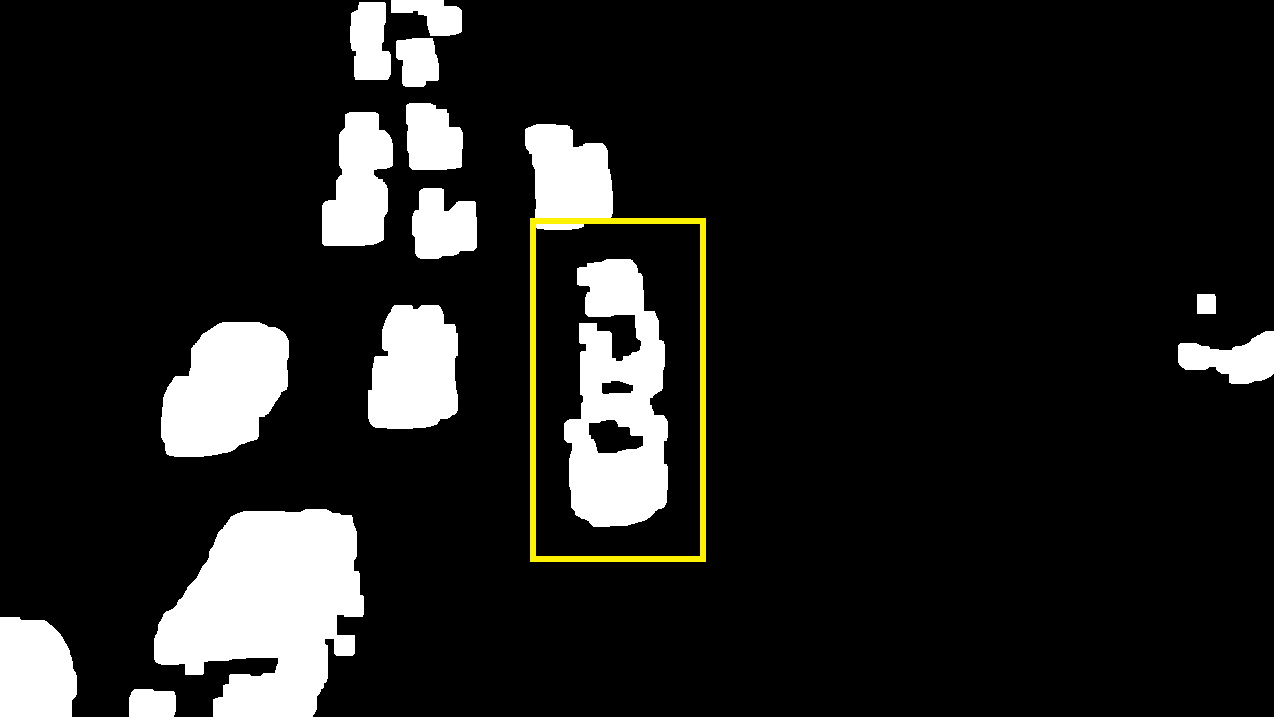
\includegraphics[width = \textwidth]{design/detection/calibration/mask}
        \caption{Foreground Mask - vehicles moving.}
    \end{subfigure}
    \begin{subfigure}[b]{0.4\linewidth}
        \centering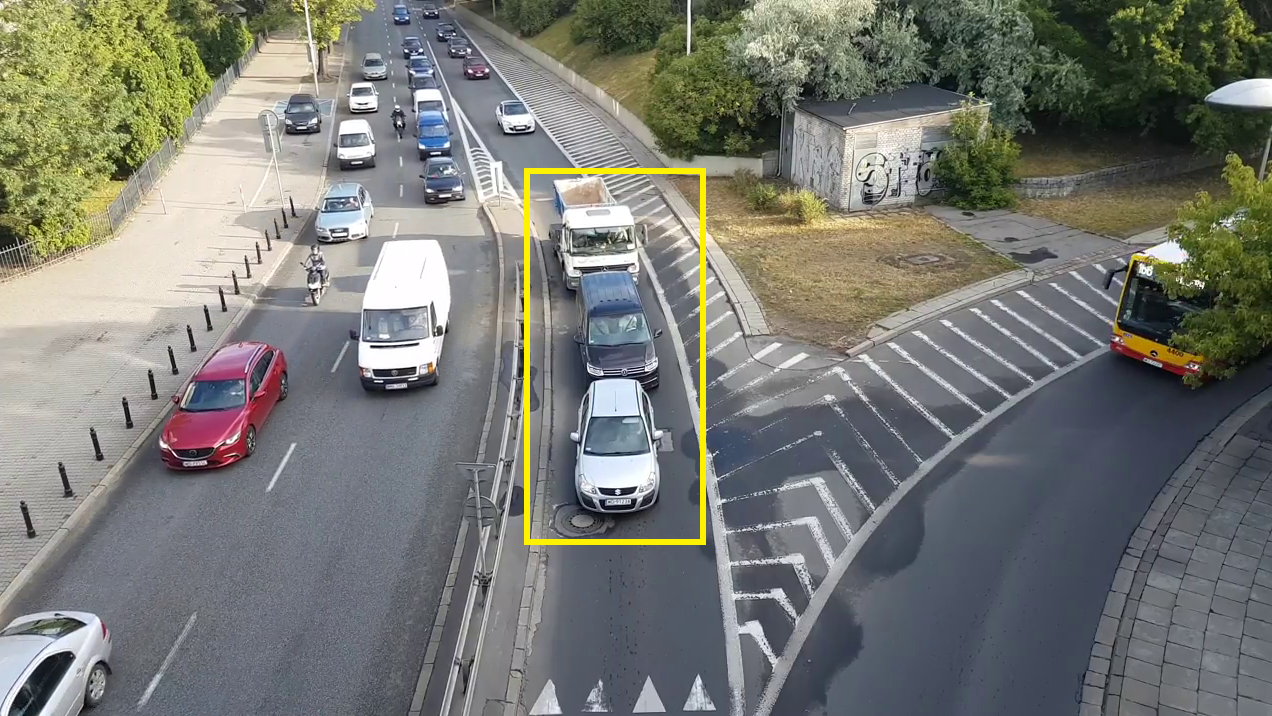
\includegraphics[width = \textwidth]{design/detection/calibration/original_adapted}
        \caption{Original Frame - vehicles stopped.}
    \end{subfigure}%
    	\begin{subfigure}[b]{0.4\linewidth}
        \centering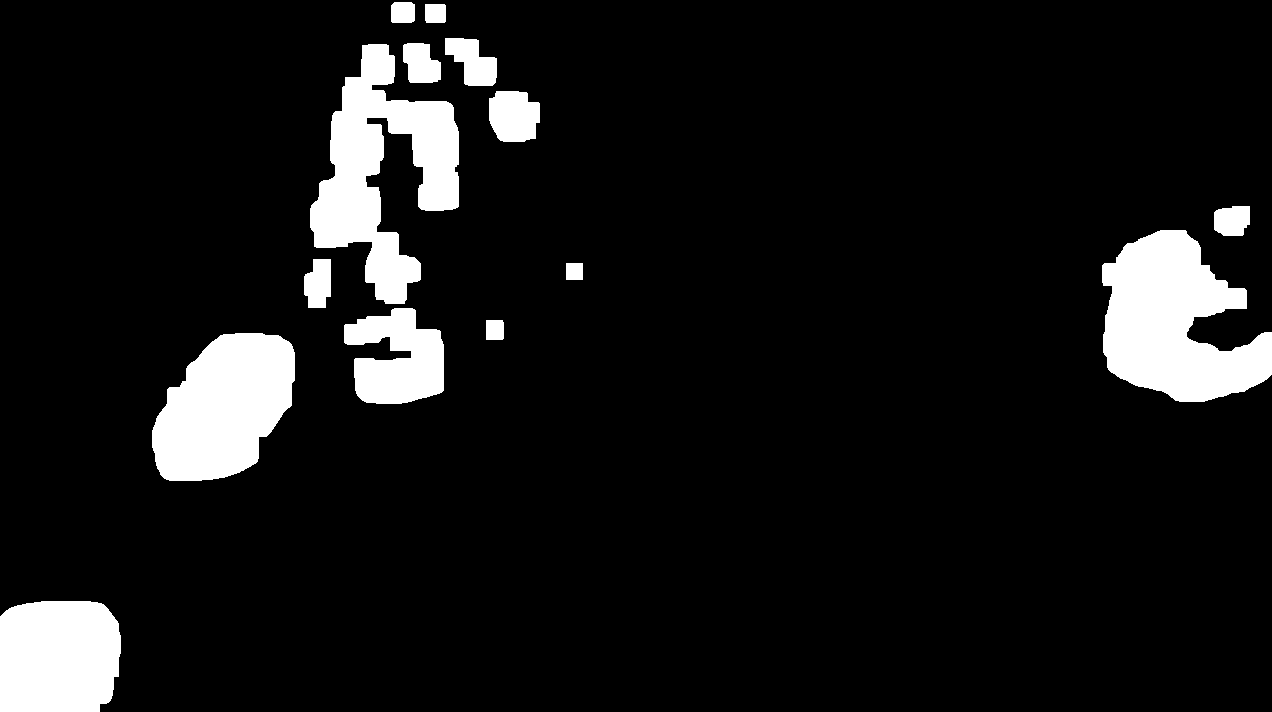
\includegraphics[width = \textwidth]{design/detection/calibration/mask_adapted}
        \caption{Foreground Mask - vehicles stopped.}
    \end{subfigure}
    \caption{Adaptation GMM background cluster. Images by Karol Majek}
    \label{fig:cluster_adaptation}
\end{figure}


